\documentclass[tikz,border=9pt]{standalone}
\usepackage{amsmath,amssymb}
\usetikzlibrary{arrows.meta,positioning,calc}
\begin{document}
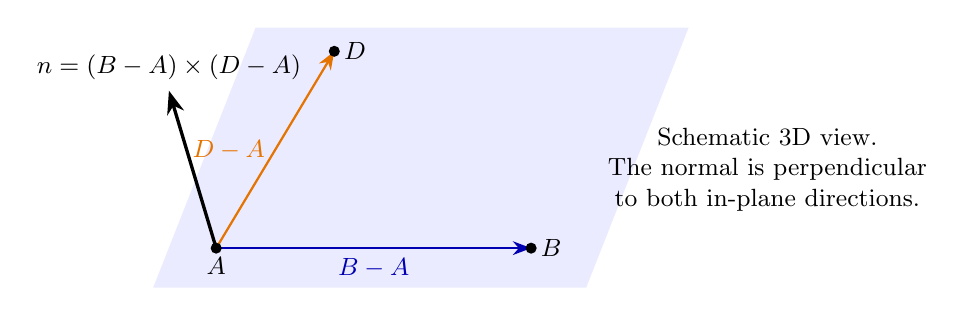
\begin{tikzpicture}[font=\small,arr/.style={-{Stealth},thick},box/.style={draw=blue!55!black,rounded corners,fill=blue!4,align=center,text width=2.9cm,minimum height=1.05cm}]

\coordinate (A) at (0,0);\coordinate (B) at (4,0);\coordinate (D) at (1.5,2.5);
\fill[blue!8] (-.8,-.5)--(4.7,-.5)--(6,2.8)--(.5,2.8)--cycle;
\draw[arr,thick,blue!70!black] (A)--(B) node[midway,below]{$B-A$};
\draw[arr,thick,orange!90!black] (A)--(D) node[midway,left]{$D-A$};
\draw[arr,very thick] (A)--(-.6,2) node[above]{$n=(B-A)\times(D-A)$};
\fill (A) circle(2pt) node[below]{$A$};\fill (B) circle(2pt) node[right]{$B$};\fill (D) circle(2pt) node[right]{$D$};
\node[align=center] at (7,1){Schematic 3D view.\\The normal is perpendicular\\to both in-plane directions.};

\end{tikzpicture}
\end{document}
